\documentclass[11pt,english,a4paper]{article}
\usepackage[utf8]{inputenc}
\usepackage[T1]{fontenc}
%\usepackage[DIV9]{typearea}
% Delete any .aux files if you get a compilation error when not using norsk
\usepackage[english]{babel}
\usepackage{amsmath,amssymb}
\usepackage{txfonts}
%\usepackage[scaled=0.85]{couriers}
\usepackage{textcomp}
\usepackage{verbatim}
\usepackage{cite}
\usepackage[pdfborder={0 0 0}]{hyperref}
\usepackage{varioref}
\usepackage[bottom]{footmisc}
\usepackage[justification=centering]{caption}
\usepackage{graphicx}
\usepackage{listings}
\usepackage{booktabs}
\usepackage{enumitem}
\usepackage{icomma}
\usepackage{ellipsis}
\usepackage{setspace}
\usepackage[expansion=false]{microtype}
\usepackage[]{algorithm2e}
\usepackage{ifikompendiumforside}
\usepackage{wrapfig}

\setstretch{1.1}
\frenchspacing
\sloppy

\hyphenpenalty=2000
\relpenalty=10000
\binoppenalty=10000
\clubpenalty=10000
\widowpenalty=10000

\setlength{\parskip}{0pt}
\renewcommand{\topfraction}{1.0}
\renewcommand{\bottomfraction}{1.0}

\setlist{noitemsep}

\lstset{language=C,
  basicstyle=\ttfamily,
  keywordstyle=\bfseries,
  aboveskip=0pt,
  belowskip=0pt,
  showstringspaces=false,
  emptylines=100,
  tabsize=2}

\lstset{emph={NULL, SAD, TRA, NUM_THREADS_SAD, TOP, LEFT, RIGHT, BOTTOM},
  emphstyle=\textit}

\setcounter{secnumdepth}{-1}

%INF5960 - Informatikk. Masteroppgave
\title{INF5960: Informatics\\Master thesis: Essay}
\author{\large{\mbox{Ingrid Grønlie Guren}}}


\begin{document}
\ififorside

% url for footnotes
\urldef\nowikidump\url{http://dumps.wikimedia.org/nowiki/latest/}
\urldef\categorytree\url{http://no.wikipedia.org/w/index.php?title=Spesial%3AKategoritre&target=Astrid+Lindgren&mode=categories&namespaces= }.
\urldef\olejohandahleng\url{http://en.wikipedia.org/wiki/Ole-Johan_Dahl}


\pagenumbering{arabic}


%%---------------------------------------------------------------------------%%

\begin{abstract}
Automatic categorization of content is an important piece of functionality in online advertising and automated content recommendations, both for ensuring contextual relevancy of placements and for building up behavioral profiles for users that consume the content. Within the advertising domain, the taxonomy tree that content is classified into is defined with some commercial application in mind and needs to somehow reflect the advertising platform’s ad inventory. The nature of the ad inventory and the language of the content might vary across brokers (i.e., the operator of the advertising platform), so it is of interest to develop a system that can easily bootstrap the development of a well-working classifier. Brokers are often not very technical and by experience will have severe problems developing training sets or otherwise contribute to the process, so any required involvement from their side has to be relatively simple. Furthermore, it is a practical requirement that the classifier can “explain” it’s classification to the broker in some way, and that the broker can have a simple way to manually override or influence the classification of known problem cases.

We explore the use of Wikipedia to develop a simple dictionary-based classifier. A dictionary-based classifier offers a simple way to “explain” the classification, and allows the classification vocabulary (i.e., the dictionary entries) to be easily edited. Wikipedia exists in a large number of languages, has a large number of article keywords covering most domains, and explicitly associates article names with categories. We describe a set of tools that automate the process of building up dictionaries that map Wikipedia keywords (or cleansed versions thereof) into Wikipedia categories (or modified versions thereof.) Creating a mapping that maps Wikipedia categories into the broker’s custom taxonomy tree is a relatively straightforward task that brokers (or people working on their behalf) are assumed capable of. We will here use the IAB taxonomy as a working example of such a custom taxonomy tree.

Given such a classifier, we describe an experiment using a real advertising platform to validate its use in real life using real data. We also provide a brief overview of related work described in the literature.
\end{abstract}

\subsection*{Introduction}
Content analysis is the task of analysing and understanding collections of text, in other word finding out what a text is about. The task can be performed by both human and computers, where both of the approaches have their advantages and disadvantages.

The concept of human content analysis is easy, where the process is to read and understand the text before summarizing the content of the text and/or categorize it into suitable categories. For instance would an article about Astrid Lindgren (the famous Swedish children books' author) probably be summarized as an article about a famous Swedish children books' author and categorized as an article about authors of children books and Swedish people. Two of the main disadvantages of human content analysis is that the task is time consuming i.e., it takes time to read and understand the article and requires resources because some articles needs experts for understanding the content. 

%first has to be read and understood and then we could summarize the content of the text or categorize it under relevant topics.
Computer content analysis is based on a different approach; instead of reading and understanding the text, the computer looks for words that is known and uses these words to find the content of the text. There are some issues with computer content analysis that are important to handle. The first is that the computer cannot define its own categories, but needs a predefined set of possible categories. It is a lot easier to ask the computer "Is the article about a children books author?" than to let the computer find this possibility itself. The other issue is to decide what words are important and useful for deciding the categories of a text. 

%The computer content analysis is an automatic categorization process, where we want to find words that help us define the categories of the text. 
The first issue can be solved by defining a set of categories that we want to categorize text to. There are some requirements that needs to be satisfied for our set; the set has to so large that all relevant texts could be placed under a category, and the set has to be so general that common texts would be categorized together. We also have to make sure that the set of categories is defined so that a text is not categorized under conflicting categories, for instance the category "sport" and the category "not sport". 

A predefined list of keywords is ideal for dealing with the issue of deciding what words are useful for categorizing. If the keywords already has a mapping


The thought about keywords is that there are some words that are more likely to give away the content of an article. If an article mentions Pippi Langstrømpe (the main character in lots of Astrid Lindgren's children books) is the probability for the article to be about Astrid Lindgren larger than if the articles does not mention the name. 

The main reason for using keywords is


than for a computer where the content has to be stored in categories


Our overall goal is to make the computer understand the interests of the user by understand texts that the user is interested in, for instance articles read or text on web pages visited. 


the performance by humans could be 

Then human task of content analysis 


i.e., 



The overall goal is to let the computer understand the interests of the user by understanding the content of text. 

The easiest way to perform content analysis for a computer is to find specialized words in texts and find out what these words mean. 

**Some words are more likely to reflect the content of an article than other. 




do categorization of content. 

, and our goal is to make the computer understand different texts. 

. The purpose of understanding the text  




a useful approach for improving user experience or advertising. User experience can be improved by letting the computer know the interests of the user, and therefore make better suggestions. Advertising can be improved by directing the advertisement towards users that are more likely to become customers or consumers. 


On way of achieving content analysis is through contextual classification.  The classification should be an automatic process since there are lots of data to process, and to make the classification possible in all languages with only small changes. 

%Taking use of Wikipedia as a knowledge base would 

%\subsection*{}

%It is almost impossible to find a proper model for large amounts of data if the model is based on training sets, and we will therefore use 
%Problemet: Innnholdsanalyse
%-> brukes i advertising-formål

%kontekstuell  og behavioral reklame -> mer penger for
%mye data -> autmatisk klassifisering. 

%mange teknikker, lager en modell
%utfordinger: umulig a lage treningssett. 
%Teknikk som er lett å bootstrappe, ikke krever noe fra kunden, gir en output som kunden kan forstå, enkelt å variere


%The technique used for 

%lett å bootstrappe og mange språk -> wikipedia er egnet for dette formålet. 


%User experience can be improved by letting the computer know what the interests of the user. There are different ways of achieving %knowledge about the user behavior. One of these approaches is to use contextual classification which is the topic of this article.  

% WHY
%Improving user experienceere
%Advertising. 


%Improving user experience is relevant in many contexts, for instance advertising

% HOw: 


%but this article will discuss the approach of using contextual classification. 



%focus on using contextual classification for 

%User experience can be improved if the computer knows the interests of the user. If the computer for instance understands the content of an article, it could use this to find similar articles within the same topic. One way of finding similarity between documents is by classifying the documents together so that articles of the same topics are linked together.  

%This paper describes the usage of classification of Wikipedia to understand the content, and how this could improve the overall user experience. The article will start with an introduction about Wikipedia and classification in general. The main part of this paper will cover the usage of Wikipedia as a knowledge base for classification, with the purpose of improving the user experience. The paper will discuss some of the applications of the different classification approaches.

%before covering a discussing of the classification applications and a summary of a classification approach.subsection*
I\subsection*{Introduction}

There are a lot of challenges for our classification technique. The result from our classification should be easy to understand for the users of the result, including the non-technical users. This means that the result of our classification should not be measured by some numbers, but should instead be "translated" to a understandable result. 



Finding a good automatic classification has


The paper will start with a short introduction to Classification followed by a short introduction to Wikipedia and why this is a good knowledge base for our classification problem. 

\subsection*{Classification}
Classification is defined as 
\begin{quote}
"[...] the problem of identifying to which of a set of categories (sub-populations) a new observation belongs [...]" %\footnote{http://en.wikipedia.org/wiki/Statistical_classification}
\end{quote}
In other words, classification is given as the task of sorting elements together given some logic structure. There are three different approaches to achieve classification (see also figure \ref{fig:classification_approaches}): 
\begin{itemize}
\item \textit{Manual classification:} Experts decide the class of the input
\item \textit{Rule-based classification:} Rules decide what classification to achieve
\item \textit{Statistical classification:} Based on some training data set. 
\end{itemize}
The manual classification is the one that usually produce the best result, but is both time consuming and tedious when there are lots of classes and input. The purpose of using machine learning in classification is therefore to automate the repetitive task of deciding the category of some input.

\begin{figure}
\centering
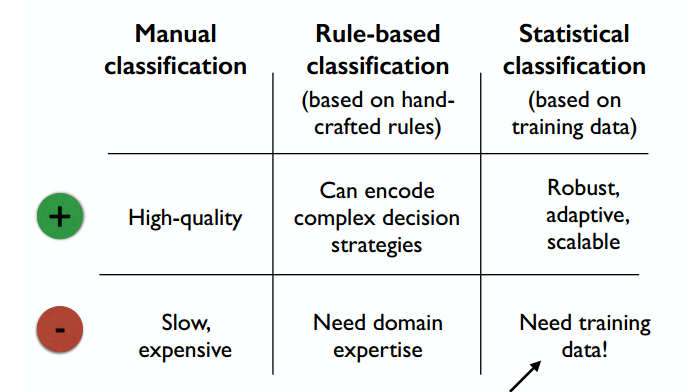
\includegraphics[height=6cm]{classification_approaches}
\caption{Advantages and disadvantages with different classification approaches}
\label{fig:classification_approaches}
\end{figure}
Machine learning is defined as the technique of teaching the machine how to behave, where our result usually is a process where we learn the machine how to behave given some input. The process is about finding patterns or to predict, and the goal for the process is that the behavior becomes as optimal as possible. 
There are three approaches of learning within machine learning: supervised learning, reinforcement learning and unsupervised learning. 
\begin{itemize}
\item \textit{Supervised learning} is a technique where the machine is given a training data set. The training data set in supervised learning is a data set that contains the correct output in addition to the input we want to classify. The classifier can use this data to train the classifier so it returns the wanted output.
\item \textit{Reinforcement learning} is a machine learning approach where the machine receives some feedback about the result of the actions made.   This can either be after each action, or at the end. 
\item \textit{Unsupervised learning} is the task of trying to find a hidden structure in labeled data. The difference is that the classifier receives no feedback about the result. 
\end{itemize}
There are of course advantages and disadvantages with all approaches listed above, and which method to choose is decided by the problem definition.

In this classification problem is a unsupervised classification preferable. Trying to solve the problem with supervised classification would lead to some problems; it is almost impossible to create a training set for such a large data set that we could base our model on and it is difficult to adjust the model to fit changes. 

%Classification as a part of machine learning, is the process where we give some input to the machine (at set of objects) and want to get outputs (the categories) in which they belong. The process is to find the function, also called classifier, that predicts the output for any input. This is usually written as

%\[\gamma: X \rightarrow Y \]

%Classification is  usually either supervised, where we give a training set with the correct output, or it is unsupervised, where the classifier tries to find common features in the data and categorize based on this. 



\subsection*{Wikipedia and classification}
Wikipedia is a free, online encyclopedia and online community\footnote{\url{http://no.wikipedia.org/wiki/Wikiedia:Hva_Wikipedia_ikke_er}} that was created by Jimmy Wales in 2001. The encylopedia is edited by the Wiki-principle, which means that everyone can create and edit articles,\footnote{\url{http://www.snl.no/Wikipedia}} and the articles are structured within language. 

To understand the importance of Wikipedia, it is also worth mentioning that the web page has been ranked as the fifth globally most important web page \footnote{New York Times, February 2014} and that there are more than 30 million articles and almost 500 unique users a motnth. 

%There are a total of  287 languages, but the number of articles available in a language depends on the language of the editors. 

%Wikipedia is one of the largest and most important web pages (ranked as the fifth globally most important web page by New York Times in February 2014), and has a total of 30 million articles and almost 500 million unique users a month.\footnote{\url{http://en.wikipedia.org/wiki/Wikipedia}, date: 21th of May, 2014} According to Wikipedia there is between 25,000 and 60,000 page requests per second per day depending on the time of the day. This makes Wikipedia one of the most visited pages, and also puts pressure on the page, to make sure it is maintained and updated at all time. 

\subsubsection{How is it structured?}
The structure of Wikipedia is similar to a web, where articles with similarities are linked together. Since Wikipedia is language-based, articles only link to other articles within the same language. Wikipedia does also have a category structure, where all articles are classified under at least one category. A category could have articles, but could also have subcategories, where the subcategories have their own articles and subcategories. The categories form a large category tree where articles are put under the most describing category. For instance will Ole Johan Dahl \footnote{\olejohandahleng} (Norwegian computer scientist) be placed under the category \textit{Norwegian computer scientists} instead of the parent category \textit{Computer scientists by nationality}.

Figure \ref{fig: subcat_lindgren} is an example of a structure for the category \textit{Astrid Lindgren}, a famous Swedish author of children books. The figure is an example of a the tree structure of categories. The figure shows that the category \textit{Astrid Lindgren} has 7 pages directly under the category, and 3 subcategories: \textit{Astrid Lindgrens karakterer} (7 pages), \textit{Astrid Lindgrens bøker} (9 pages) and \textit{Pippi Langstrømpe} (16 pages).  This means that there are indirectly 39 pages under the category \textit{Astrid Lindgren}. 

%is created and how it is fetched from the page for category information.\footnote{\categorytree}

\begin{figure}
\centering
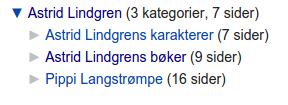
\includegraphics[height=3cm]{Dumps/imgs/Kategorier-Astrid-Lindgren.png}
\caption{Subcategories of the category \textit{Astrid Lindgren}. }
\label{fig: subcat_lindgren}
\end{figure}

An article in Wikipedia can be categorized under more than one category. This does not necessarily mean that the categories are equal, but that the article has content that can be categorized under more than one category. Some of these categories might therefore be unnecessary or redundant, where the the combination of two specialized categories might not provide more information. An example of a specialized category is the article of \textit{Ole Johan Dahl}. Some of the article's categories are showed in figure \ref{fig: olejohandahl_categories}. This is an example of an article where the categories provide the same information, i.e., we already know that he was from Norway since he is in the category \textit{People from Mandal, Norway}, so it would be enough to add that he was a computer scientist instead of specifying that he was a Norwegian computer scientist. 

\begin{figure}
\centering
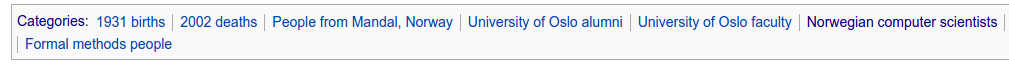
\includegraphics[width=\textwidth]{Dumps/imgs/olejohandahl-categories.png}
\caption{Some categories from the article of Ole Johan Dahl}
\label{fig: olejohandahl_categories}
\end{figure}


%\begin{figure}
%\centering
%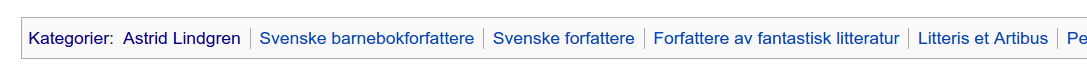
\includegraphics[width=\textwidth]{Dumps/imgs/Astrid-Lindgren-Wikipage-short.png}
%\caption{Categories of the Wikipedia page "Astrid Lindgren"}
%\label{fig: wikipage_lindgren}
%\end{figure}

Removing categories that are too specified is a way of avoiding redundancy in the categories. I have noticed that the category could be grouped into there different types of categories. The first type is the categories that are very general, for instance \textit{sport} or \textit{history}. The second type of category is the category that is only used to sort its subcategories. The category \textit{Computer scientists by nationality} is an example of the second type of  category where there are no direct articles, but only subcategories that are more describing. Such a category will therefore be less useful in our classification. We could either remove the category, but might then loose information. We could flat the category tree, where all the subcategories' articles will be moved to the parent category. The last type of categories that I have noticed is the category that is specified towards one or more articles. Some of these might not be useful, for instance if they are specified towards only one article. 


%Content on Wikipedia is structured like a web with lots of articles that links to each other. Articles in Wikipedia is language-based, so that articles in one language link to other articles in the same language. 
%A criticism against Wikipedia is that some languages have more articles mainly because there are more people who know the language (see Figure \ref{fig:languages}.
%To make browsing easier, similar articles are structured in a similar fashion, so that users may see the resemblance between the articles. Articles are also linked together, where words with their own Wikipedia page (often places, persons or events) have links to the corresponding page. 

%\begin{figure}
%\centering
%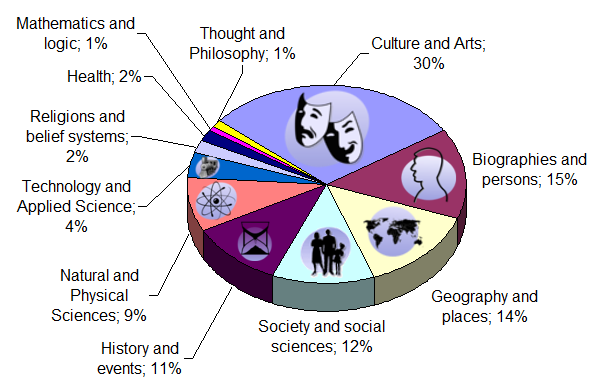
\includegraphics[height=8cm]{Wikipedia_content_by_subject}
%\caption{Pie chart of Wikipedia content} %\footnote{\url{http://upload.wikimedia.org/wikipedia/commons/5/54/Wikipedia\_content\_by_subject.png}}}
%\label{fig:pie_chart}
%\end{figure}


%Wikipedia contains lots of information on various subjects. Figure \ref{fig:pie_chart} is a pie chart from January 2008 that shows the various contents of Wikipedia. There are, as we can see, a lot of articles about everyday interests like culture and arts, which is one of the main reasons why Wikipedia is in such common use. Two of the most common usage areas are listed below, 
%\begin{itemize}
%\item \textbf{At home}: Several articles on Wikipedia are written about subjects we encounter in everyday life. This is also a reason that Wikipedia is such a large online web page, and is almost always among the top ten results if we search for something online, but only if the search is not too specific. %Wikipedia is also quite common to use in discussions or. 
%\item \textbf{Studying or at work}: Wikipedia is very useful as an encyclopedia, which means that it is an easy tool to use when looking for facts or information about subjects. Lots of universities and schools discourage students from using Wikipedia as their primary source, reasoning that articles from Wikipedia could be written by anyone. 
%\end{itemize}

%\subsection*{Classification}
%\subsection*{What is classification?}

\subsubsection*{Why use Wikipedia}
There are many reasons to use Wikipedia as a knowledge base for classification.


\subsection*{Classification of Wikipedia}
The general hypothesis for the thesis, is as mentioned before: 
\begin{quote}
%Knowing what the interest of the users might help us improve the user experience. 
"User experience might be improved if we know what the user is interested in. "
\end{quote}
The question is how to know what the user is interested in, which could be determined by classification. The computer might be able to guess the user's interest by first classifying the content. When receiving the user's behavior, it could then try to analyze it, and find similar content within the classification group that might interest the user. There are many fields where this approach is useful, but some of the main fields are: 
%For finding out whether the classifcation has impr
% the purpose of this is .. 
% Den praktiske delen av oppgaven min, vil være å anvende klassifisering av Wikiedpia. 
%There are many fields where classification can be useful, and I have listed some of them below. 
\begin{itemize}
\item \textit{Similar articles}: It is easier to recommend other articles to a user if we know the content of articles that the user was interested in. If a user is reading an article about one topic, there is a great chance that the user might be  interested in another article of the same topic rather than something completely different. 
\item \textit{Advertising}: If we know what the user is interested in, then it is possible to use this to suggest products that the user might be interesting in. This can be an advantage for advertisers that want to sell their products, and users that might get recommendations of products of their interest. 
\item \textit{Searching}: Search engines will return better search results if they know the content of articles or web pages. This can give better results to the users.  
\end{itemize}
% It is essential to know what the user is browsing, to know the interest of the user. The idea is to use classification to categorize articles or web pages based on content. 

An approach for understanding the content, is to use Wikipedia as a knowledge base. A knowledge base is a set of sentences where each sentence represents some assertion about the world.%\footnote{The world is here given as } 
\footnote{Artificial Intelligence, A Modern Apprach. Stuart Russell, Peter Norvig. Third Edition, Pearson New International Edition, p. 207} If Wikipedia can be categorized, it could be used to look up words in articles and use this to categorize the articles. There is also a chance that words with their own Wikipedia page is more relevant for categorizing the article than words that don't. This can be used to better understand the content of articles or web pages. 

\subsubsection*{}
The practical part of my thesis will be a classification of Wikipedia, where Wikipedia will be the knowledge base to make sure that similar content are grouped together. There are different approaches in how to create a classification group as discussed above, but the result should be the same. Given some user behavior, the program should be able to respond with possible behaviors that the user might want to consider. An example is recommending similar articles for a user given some article already read, where the recommended articles could be within the same topic or other articles with same content. 

The easiest way to test the results, is by looking at the behavior of the users, or at the user experience. This will of course differ depending on scenarios, but could in many cases be tested. If users are looking at articles and choose to click on articles recommended by the classification, a conclusion could be that the classification has succeeded in recommending articles. It would in addition also be relevant to see whether the users are interested in continuing to look at or read the article or not.  

The main reason to use Wikipedia as the knowledge base, is that Wikipedia is rapidly and frequently updated. Lots of articles on Wikipedia is updated right after events occur. Examples are the Wikipedia page of Catherine (Duchess of Cambridge) which changed name right after the vows in the royal wedding in 2011 or the Wikipedia articles about soccer teams right after the final matches in the Champions League. Another benefit of using Wikipedia is the principle that everyone can create articles or edit them. 
In my opinion, Wikipedia also has two disadvantages:
\begin{itemize}
\item \textit{Anyone can edit}: This means that the user doesn't know the author of a given article and the article might be incorrect or have missing information. 
\item \textit{Encyclopedia}: Even though Wikipedia is an online encyclopedia, there are always some articles that are missing, which might make the classification incomplete.  
\end{itemize}
To compensate for these disadvantages, Wikipedia has two approaches; poorly written or articles with lacking information can be flagged so that other authors can look at it, and users can request topics that does not have an article yet. 

%\subsection{Applications}
When using Wikipedia as a information source, we can classify in different ways. One of them is as described above, where we give categories to the articles so that they are sorted on a topic. This could be used to get information about the topic presented in articles that link together. 

Another application is clustering, which is the task of grouping a set of objects so that similar objects are grouped together. This is useful since many topics are mentioned together and a user interested in one topic might be interested in other topics that are usually mentioned together. 

A third application is to make a map between keyword and categories. This could link some keywords against some topics, for instance could specific soccer players link towards articles about football. 


\section*{Similar work}
I have read the article "Entity Extraction, Linking, Classification, and Tagging for Social Media: A Wikipedia-Based Approach"\footnote{\url{http://pages.cs.wisc.edu/~anhai/papers/doctagger-vldb13.pdf}}. This article writes about a classification problem, where tweets are classified with Wikipedia as the knowledge base. 

The article describes the goal as classifying tweets automatically with machine learning so that tweets with similar content will be classed together. %The use is to know what the tweet is about so that users with 
The authors chose to use Wikipedia as a knowledge base since it is the largest online encyclopedia we have, and because it is based on volunteering. Wikipedia is also constantly crawling which means that they build a fresh, dynamic and timely knowledge base.  

The first step mentioned in the article, was the step of preprocessing the tweets. The preprocessing started with detecting the language of the tweets and then cleaning them (remove everything that is not text) and tokenizing them (separating sentences into tokens, which is defined as a sequence of characters, usually words). The second step was to extract mentions. Mentions were given on the form ($m_{i}$, $n_{i}$, $s_{i}$) which corresponds to: 
\begin{itemize}
\item $m_{i}$: sting in the tweet we refer to
\item $n_{i}$: node in the knowledge base
\item $s_{i}$: score of the node 
\end{itemize}
All of the tokens which are connected to a node in the knowledge base are in this first step considered relevant, and we sort them. 

The next step is to filter the mentions where all unnecessary mentions are dropped. The mentions that are filtered, are based on a set of hand-crafted rules, and then the result is scored again. The gaol is to redo the classification and tagging once again to improve the results further.

\subsubsection*{The evaluation}
One of the most important steps of classifying is the evaluation phase. Evaluation of classifying should be done by humans. Someone will have to look through the results and see how well the classification has been done by comparing the \textit{correct} result with the \textit{predicted} result.

The article concludes that the tweets that were easiest to classify were about people (see Figure \ref{fig:classification_entities}). This is probably because famous people have their own Wikipedia page, which is easy to match the tweet. The most difficult, on the other hand, was products which seldom have their own page  if the tweet is very specific. 


%The goal of the program is to link tweets to Wikipedia articles and then use this to classify tweets.

%The approach start with linking the entities in the Knowledge Base because common words will have

%The process of classifying the tweets: 
%Preprocess: where the written language is detected and the tweet is cleaned and tokenized
%Extract mentions: Returns links to the odes in the Knowledge Base
 %(here they used a dictionary approach that contains a prefix map (prefix, nodeID, stop?). This will look for matches in the knowledge base, and will try to get as long prefix as possible to match the current string. 
%Filter and score mentions: The approach drops all unnecessary mentions (like stop words we use in search technology) and give all the rest a score. The first scoring considers if it's a noun, popular homonym or appears in a title



%classify and tag tweets:  Before classifying the tweets are all mentions given on the 

%What is difficult to classify?
%The result of the paper shows that the tweets that were most difficult to sort where those about products (15.38), Social Sciences (14.29)

%The easiest to classify where the categories People

%the reason for this might be that famous people usually have their own Wikipedia page, but prodcuts

\begin{figure}
\centering
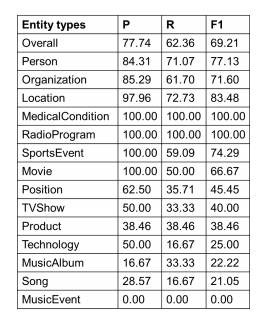
\includegraphics[height=8cm]{Classification_entities}
\caption{The accuracy of our system for extraction and linking. P is the precision, R is the recall and $F_{1}$ is the $F_{1}$-score.} %linking\footnote{\url{http://pages.cs.wisc.edu/~anhai/papers/doctagger-vldb13.pdf, page 8}}}
\label{fig:classification_entities}
\end{figure}


\subsection*{Summary}
This paper has given an introduction of some applications of Wikipedia and why it might be useful in classification and as a knowledge base. One of the main advantages mentioned is that there are lots of editors and users of Wikipedia which forces the encyclopedia to be up to date at all times. Another advantage is its structure where pages with similar content often are linked together, which makes a natural classification of the content. My thesis will focus on this hypothesis and see if the user experience can be improved by applying classification.

%Some advantages are quite clear, for instance that there are lots of editors 
%we have seen that Wikipedia can be useful for classification bevause it has a lot of advantages, for instance: lots of editors and users - > advantage of being up to date. It also have a useful structure that links relevant pages together. 


\bibliography{mini}
\bibliographystyle{norplain}
%\newpage
\section*{References}
\begin{itemize}
\item \url{http://en.wikipedia.org/wiki/Statistical_classification}
\item \url{http://www.uio.no/studier/emner/matnat/ifi/INF3800/v14/undervisningsmateriale/lecture_090414-print.pdf}
\item Introduction to Information Retrieval, Author by Christopher D. Manning, Prabhakar Raghavan, Hinrich Schütze. Cambridge University Press; 1 edition (July 7, 2008)
\item Artificial Intelligence, A Modern Apprach. Stuart Russell, Peter Norvig. Third Edition, Pearson New International Edition, p. 207
\end{itemize}


%%---------------------------------------------------------------------------%%



\end{document}
